%\section{Requirements specification}
\chapter{Requirements specification}

Be more precise about what the system should and should not satisfy.
Be sure to use the vocabulary introduced in the problem analysis.


\subsection{Timeplan}
Our timeplan follows an agile development system called waterfall.
The waterfall system is a sequential design process.
It is designed to get through the project phases and have a product as soon as
possible. The phases in our project can be seen in the figure below.

Project management
When the waterfall ends and we still have time
we will go back to the start and check for new requirements
and the whole waterfall process starts again.
The report is both written seamlessly and separately in the end of the project,
therefore it does not has to be illustrated, as it will create confusion.


Tasks management
When providing the tasks we use the timeboxing method.
This method increases the productivity significantly.
Timeboxing works by breaking a big task into smaller tasks with better manageable time frames.
It kinda works like a stopwatch.


\begin{figure}[h]
  \centering
  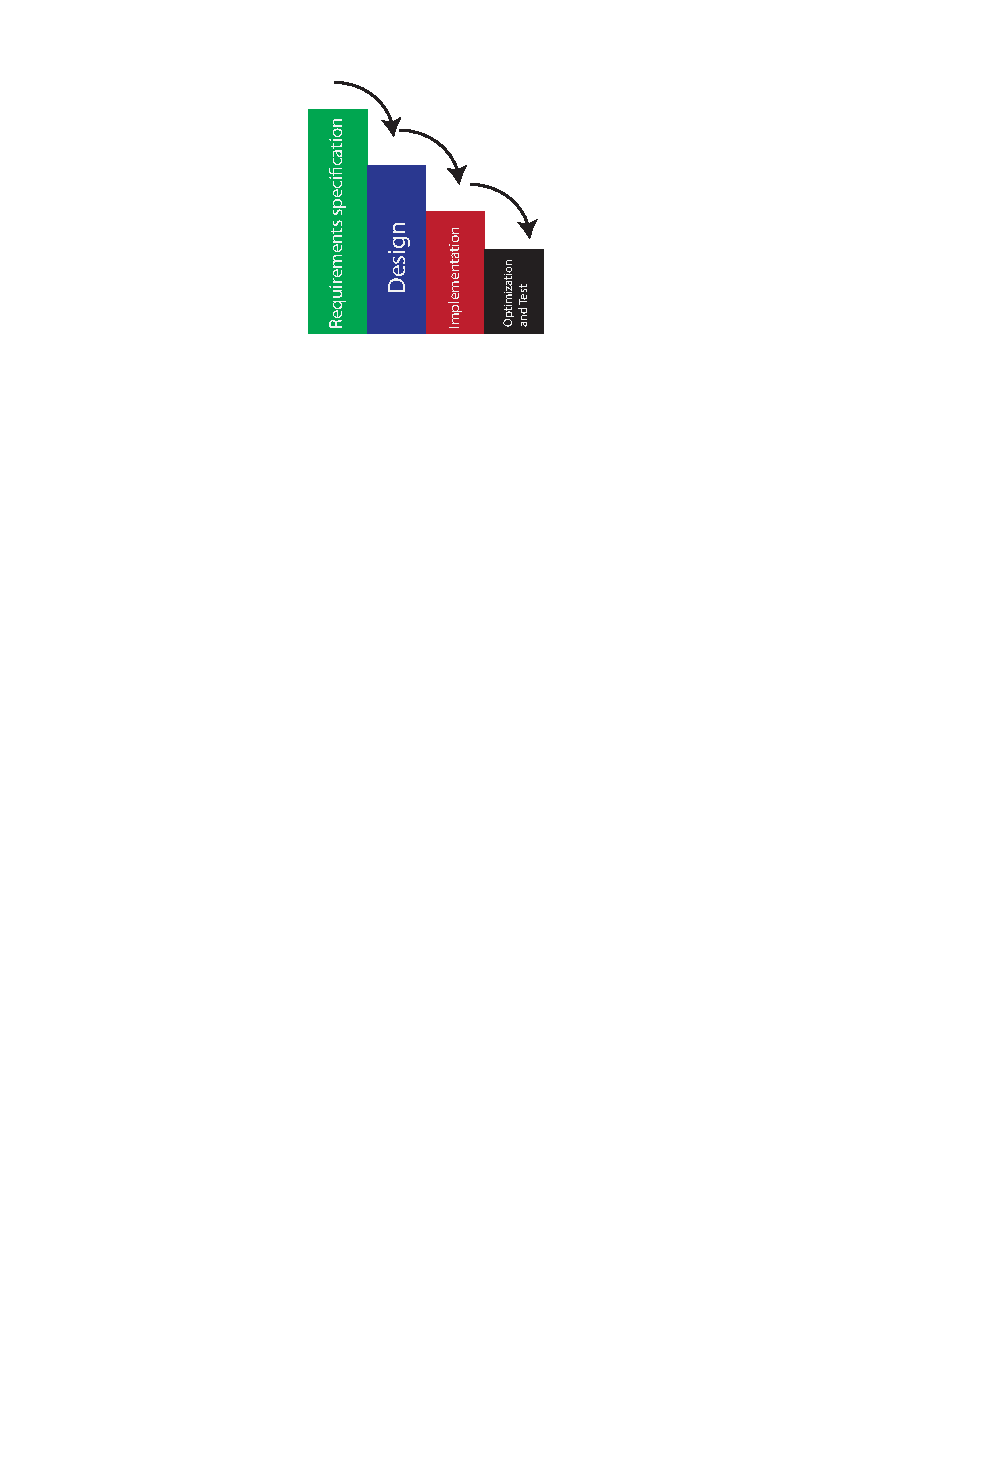
\includegraphics[scale=0.6]{Figures/Waterfall}
  \caption{An overview of the waterfall timeplan.}
\label{fig:Waterfall}
\end{figure}

